\documentclass[../main]{subfiles}
\ifSubfilesClassLoaded{
    \dominitoc
    \tableofcontentsfile
	\pagenumbering{arabic}
    \setcounter{page}{1}
	\setcounter{chapter}{6}
	\addbibresource{../Biblio/biblio.bib}
}{}

\begin{document}
\graphicspath{{../06b-Analyse-2D}, {06b-Analyse-2D}}

\chapter{Extension des mécanismes d'auto-organisation aux cartes en deux dimensions}\label{chap:analyse2D}

\minitoc

\section{Introduction}

Dans les chapitres précédents, nous avons étudié les propriétés d'organisation de cartes en une dimension d'une architecture de cartes CxSOM.
L'étude des cartes en une dimension nous offrait un cadre de représentation facile pour la mise en valeur des mécanismes d'organisation et d'apprentissage des relations entre les entrées.
Cependant, les cartes auto-organisatrices généralement utilisées en pratique sont des cartes en deux dimensions. 
Alors que des cartes 1D extraient une représentation en 1D de l'espace d'entrée, les cartes 2D ajoutent une dimension de représentation tout en restant relativement peu coûteuses en calculs. 

Nous avons étudié des architectures de deux et trois cartes 1D~; nous nous intéresserons dans ce chapitre à des architectures de deux et trois cartes 2D. 
Le modèle CxSOM tel que présenté au chapitre~\ref{chap:modele} est adapté à des cartes de dimension et de voisinage quelconque. 
Les expériences présentées dans ce chapitre ne nécessitent pas d'adaptation spécifique de l'algorithme.
L'objectif de ce chapitre est de présenter comme les comportements d'organisation identifiés sur les cartes en une dimension se traduisent sur des cartes en deux dimensions.
Ces exemples nous permettront d'identifier des limites et perspectives pour le passage des cartes 1D à 2D dans des architectures CxSOM.

\section{Présentation de l'expérience}

\subsection{Architecture de cartes 2D}

\begin{figure}
	\centering
\includegraphics[width=0.7\textwidth]{grid_torsion.pdf}
	\caption{Exemples d'organisation de cartes classiques sur des entrées présentées dans $[0,1]^2$. 
	La carte de gauche est \og bien dépliée \fg{}~: deux entrées proches sont représentées par des BMUs proches. 
	Au contraire, la disposition de droite présente un point de torsion. Cette disposition peut évoluer vers une carte bien dépliée ou vers un état stable qui présente encore un point de torsion, en fonction des paramètres d'apprentissage. Dans ce dernier cas, la carte est toujours organisée sur chaque morceau de cartes, mais n'est pas totalement ordonnée. \label{fig:torsion}
	}
\end{figure}
L'architecture de cartes en deux dimensions est construite sur le même principe qu'une architecture de cartes 1D, le modèle présenté au chapitre \ref{chap:modele} étant valable pour n'importe quelle dimension de carte.

Les n\oe{}uds d'une carte sont positionnées sur une grille carrée de taille $100 \times 100$ et indexés entre 0 et 1 sur chaque dimension. Nous notons cet index $\mathbf{p}\m{i} = (p\m{i}|_x, p\m{i}|_y)$ sur les figures. 
Chaque carte possède donc une couche de poids externes $\w\ext \in [0,1]^2$ et une couche de poids contextuels $\w_c \in [0,1]^2$.
L'entrée contextuelle correspond à la position du BMU de l'autre carte. Il s'agit des positions 2D $\mathbf{p}\m{2}$ pour la carte $M\m{1}$ et $\mathbf{p\m{1}}$ pour la carte $M\m{2}$. 
Les activités $a_e$ et $a_c$ sont calculées par une activation gaussienne~:
$$a_e(\inpx,\mathbf{p}) = \exp(\frac{||\inpx - \w_e(\mathbf{p}) ||^2}{2\sigma^2})$$
de même pour $a_c$.
La norme utilisée est ici la norme euclidienne, que ce soit dans l'espace d'entrée et dans l'espace des positions de la carte. Les fonctions de voisinage sont également définies à partir de la norme euclidienne dans l'espace des positions d'une carte.

La caractérisation de l'organisation dans une carte auto-organisatrice en deux dimensions est plus complexe que dans les cartes en une dimension. En effet, le processus de mise à jour des poids de la carte peut mener à la formation de points de torsion, comme illustré par la figure \ref{fig:torsion}, qui induisent une organisation des poids \og par morceaux \fg{}. Cette organisation avec des points de torsion préserve la continuité des poids mais dans chaque morceau de la carte, de sorte que deux poids voisins dans la carte correspondent à des entrées similaires et constituent une configuration de poids stable. Toutefois, les poids ne sont pas totalement ordonnés à l'échelle de la carte. Dans une architecture CxSOM, cela pourrait potentiellement poser un problème pour l'utilisation de la position du BMU en tant que représentation de l'entrée~: deux entrées proches peuvent avoir un BMU éloigné dans la carte.

Dans les expériences de ce chapitre, nous avons cherché faire en sorte d'éviter de tels points de torsion dans les poids externes, afin de simplifier la compréhension des mécanismes d'organisation.
Pour cela, nous laissons les poids externes s'organiser de façon préalable sur 1000 itérations à partir des activités externes, sans prendre en compte les poids contextuels. Cette pré-organisation est réalisée en prenant un grand rayon de voisinage $r_e = 0.5$.
Ce rayon de voisinage introduit une grande élasticité, ce qui permet de pré-répartir les poids externes sur les entrées externes en évitant de former des points de torsion. Après cette étape préalable, nous réduisons le rayon externe à $r_e = 0.2$ et effectuons l'apprentissage des poids externes et contextuels comme décrit dans le modèle CxSOM. Les poids externes affinent alors leur apprentissage. Cette étape ne change pas fondamentalement le comportement des cartes, étant donné que la différence d'échelle entre les rayons externes et contextuels permettait déjà aux poids externes de s'organiser plus rapidement que les poids contextuels, mais elle aide les poids externes à ne pas former de points de torsion.

De plus, l'organisation et la convergence des poids externes n'est pas assurée en 2D lorsque l'on prend un rayon de voisinage constant, ce qui est le cas dans CxSOM.
Des travaux ont prouvé la convergence des SOM en une dimension \cite{Cottrell1998TheoreticalAO}, mais seulement partiellement pour les cartes en deux dimensions, même lorsque les paramètres d'apprentissage sont décroissants \cite{flanagan_self-organisation_1996}. En pratique, la convergence des poids des SOMs en deux dimensions est bien observée avec un rayon de voisinage décroissant, mais aucun travail à notre connaissance n'a étudié la convergence de SOMs 2D lorsque les rayons restent constants. La convergence des poids des cartes est donc une propriété à vérifier expérimentalement en deux dimensions.


\subsection{Modèles d'entrées}

\begin{figure}
	\includegraphics[width=\textwidth]{sphere_inputs_colormap.png}
	\caption{Transformation de la sphère 3D paramétrée par $U$ vers un espace 4D. La rotation permet de répartir les coordonnées des points sur les quatre dimensions sans modifier la structure des entrées. Les modalités considérées sont des valeurs 2D $\inpx\m{1}$ et $\inpx\m{2}$.
	La couleur de chaque point des figures fait référence à la valeur de $U$ correspondante, dont la disposition est présentée figure de gauche. Plusieurs valeurs de $U$ différentes permettent de générer une même valeur de $\inpx\m{1}$. Par exemple, $\inpx\m{1} = (0.5, 0.7)$ correspond à $U$ autour de $(0.6,0.3)$ (vert) ou $U$ autour de $ (0.6,0.8)$ (violet).
	\label{fig:sphere_inputs}}
\end{figure}

Jusqu'à présent, les modalités observées étaient chacune en une dimension et $U$, la variable latente également une variable 1D. Afin de complexifier la structure des entrées, nous choisissons dans ce chapitre d'utiliser des entrées dont chaque modalité est en deux dimensions, et dont le modèle latent $U$ est également 2D.
Nous analyserons des architectures de deux et trois cartes, et des modèles d'entrées dans lesquels l'ensemble des entrées externe $\mathbf{X}$ est de dimension 4 ou 6.

Nous choisissons un premier modèle d'entrée dans lequel une même valeur de $\inpx\m{1}$ correspond à deux valeurs de $U$ afin de voir si les cartes sont capables de différencier leur BMU en fonction de $U$.
Ce modèle d'entrées 4D est présenté en figure~\ref{fig:sphere_inputs}.
La variable $U$ est une valeur 2D paramétrant des points placés sur une sphère en trois dimensions.
Les deux dimensions de $U$ sont les angles paramétrant la représentation polaire de la sphère, $\theta$ et $\phi$, que nous prenons ici normalisés entre $0$ et $1$.
Pour générer les entrées, nous tirons $U = (\phi,\theta)$ dans $[0,1]^2$ selon la distribution indiquée à gauche, et en tirons un point sur une sphère en trois dimensions, de coordonnées $(x_1,x_2,x_3,0)$.
Nous changeons ensuite de repère par une rotation en 4D afin que les coordonnées du point soient distribuées sur les 4 axes de l'espace 4D. Nous effectuons également une translation et une mise à l'échelle sur chaque axe afin de normaliser toutes les coordonnées dans $[0,1]$.
Cette représentation $(x_1^\prime,x_2^\prime,x_3^\prime,x_3^\prime)$ en 4D des points de la sphère permet de définir deux modalités en deux dimensions $\inpx\m{1}$ et $\inpx\m{2}$. Sur la figure~\ref{fig:sphere_inputs}, les points sont colorés sur chaque étape par rapport à la valeur correspondante de $U$ représentée en figure de gauche.
Deux valeurs de $U$ correspondent à une même valeur de $\inpx\m{1}$, ce qui est marqué par l'existence de plusieurs couleurs de points à une même position. C'est également le cas pour $\inpx\m{2}$.
Nous sommes donc dans un cas similaire aux tracés en une dimension, et nous chercherons à vérifier si les cartes $M\m{1}$ et $M\m{2}$ apprennent à différencier les valeurs de $U$ par la position de leur BMU.


Nous utiliserons comme second modèle d'entrée 4D des points placés dans l'hypercube $[0,1]^4$. Dans cette configuration, les deux modalités 2D $\inpx\m{1}$ et $\inpx\m{2}$ sont indépendantes, rappelant la configuration des entrées prises dans le patch $[0,1]^2$ pour des modalités 1D. L'étude de configuration d'entrées indépendantes permet d'évaluer les mécanismes d'organisation qui sont liés aux règles d'apprentissage des cartes.
Nous comparerons l'organisation des cartes 2D sur cet hypercube à celle que nous avions obtenue en 1D sur le patch $[0,1]^2$. 

Nous étudierons enfin une architecture de trois cartes 2D, sur un modèle d'entrées en six dimensions construit à partir d'une sphère 3D, selon la méthode présentée en figure~\ref{fig:sphere_inputs}. Les modalités sont chacune en deux dimensions et $U$ est une variable 2D. Dans ce modèle d'entrées, la connaissance de deux modalités sur trois détermine la troisième valeur, nous permettant d'observer la capacité de prédiction de l'architecture.

\subsection{Expériences}

Ce chapitre est une série d'observations réalisées sur des architectures de cartes 2D; cherchant à généraliser les comportements observés au long des chapitres précédents sur les architectures de cartes 1D, à savoir~:
\begin{itemize}
	\item Les poids externes de chaque carte de l'architecture permettent une bonne quantification vectorielle de leur entrée externe.
	\item Les poids contextuels définissent des motifs pseudo-périodiques, qui forment des sous-cartes organisées de l'espace des entrées contextuelles.
	\item Les BMUs d'une carte se disposent en zones compactes, encodant à la fois la valeur de l'entrée externe et la valeur du modèle $U$ en formant deux échelles d'indices.
	\item Une carte ne recevant pas d'entrée externe est capable de générer une bonne prédiction de la modalité manquante dans l'architecture.
\end{itemize}

Nous nous intéressons à la réponse des cartes lors de phases de test, et présenterons l'organisation des cartes et de leurs BMU en adaptant les tracés présentées au chapitre~\ref{chap:repr} à des variables en deux dimensions.

Sur les deux modèles d'entrées 4D que nous avons décrits au paragraphe précédent, nous examinerons la disposition des poids externes et contextuels après apprentissage et la disposition des valeurs de $U$ selon la position du BMU. Nous comparerons l'organisation obtenue dans le cas des entrées dépendantes (sphère) et indépendantes (hypercube). Nous utiliserons également le ratio de corrélation présenté au chapitre \ref{chap:indicateur} pour évaluer cette organisation.
En 1D, le rayon $r_c$ détermine la taille des motifs de poids contextuels. Nous comparerons l'organisation obtenue pour différents rayons de voisinage contextuels et vérifierons la convergence de la relaxation sur ces expériences.
Nous observerons enfin l'organisation et la capacité de prédiction d'entrée dans une architecture de trois cartes 2D.

\section{Organisation des cartes sur des entrées dépendantes \label{par:orga2D}}

\subsection{Organisation des poids}

\begin{figure}[h!]
	\begin{minipage}{\textwidth}
	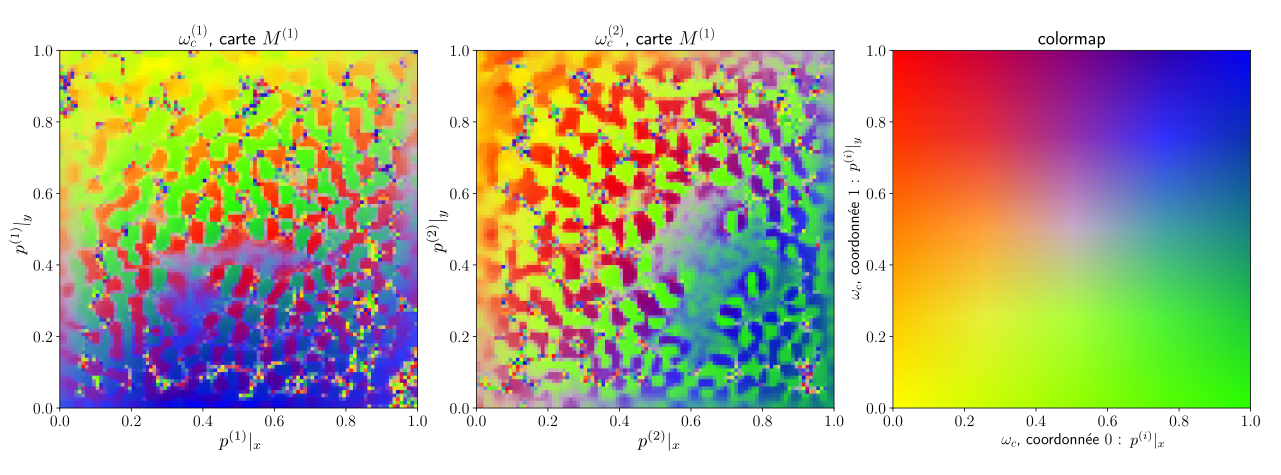
\includegraphics[width=\textwidth]{wc_rc002_afterbug_nopoints.pdf}
	\end{minipage}
	\begin{minipage}{\textwidth}
		\includegraphics[width=0.7\textwidth]{we_rc002_afterbug_step10.pdf}
		\caption{Tracé des poids externes contextuels d'une architecture de cartes, organisés sur une sphère dans un espace 4D, avec $r_e =0.2$ et $r_c = 0.02$.
		En bas, les poids externes sont positionnés en fonction de leur valeur $\w_e|_x, \w_e|_y$ et reliés aux n\oe{}uds voisins. Pour une raison de lisibilité, nous avons représenté seulement une partie des connexions, les cartes étant de taille $100 \times 100$. Le coin de position $(0,0)$ de la carte est marqué par le point rouge. Cette représentation permet d'observer directement que les poids externes de chaque carte se déplient sur les entrées externes qui lui ont été présentées, dont on retrouve le tracé en figure ~\ref{fig:sphere_inputs}.
		En haut, nous traçons la valeur des poids contextuels. Nous colorons le point situé en position $p|_x, p|_y$ de chaque carte en fonction de la valeur 2D de son poids externe. Cette représentation fait apparaître une organisation en motifs oscillants, rappelant le comportement observé en 1D.
		\label{fig:2som_s_002_wc}}
		\end{minipage}
\end{figure}

Nous étudions d'abord l'organisation des cartes sur les données tirée sur la sphère, décrite en figure \ref{fig:sphere_inputs}. 
Nous prenons dans cette première expérience les rayons de voisinage à $r_c = 0.02$ et $r_e = 0.2$, qui sont les valeurs des paramètres utilisés pour les cartes 1D.

La figure~\ref{fig:2som_s_002_wc} présente la disposition des poids externes et contextuels de l'architecture de deux cartes 2D après apprentissage.
En bas, nous représentons les poids externes dans l'espace des entrées~: un n\oe{}ud de la carte est positionné en $\w_e(\mathbf{p})$ qui est une position 2D.
En haut, nous représentons les poids contextuels de la carte sous forme de carte de coloration. Un pixel positionné en position $\mathbf{p}$ est coloré selon la valeur de son poids $\w_c(\mathbf{p})$ qui est une valeur en deux dimensions.

L'organisation de $\w_e$ montre que chaque carte représente ses entrées externes de la même façon qu'une carte 2D classique~: les poids externes de chaque carte s'étendent sur le disque dans lequel sont tirées leurs entrées externes. 
L'organisation de $\w_c$ fait apparaître des motifs oscillants spatialement dans chaque carte, qui rappellent les motifs présents en une dimension, cf. figure~\ref{fig:w}.
Ces motifs sont de taille équivalente et sont répartis sur toute la surface de la carte. 

L'organisation des poids contextuels en motifs est donc similaire entre 1D à 2D. La forme des motifs semble plus variée que sur des cartes 1D, la 2D apportant une dimension supplémentaire à l'organisation.

\subsection{Relation entre $U$ et $\bmu$ \label{par:U_bmu2D}}

\begin{figure}[t]
	\includegraphics[width=\textwidth]{U_BMU_2SOM_2D.png}
	\caption{Disposition des valeurs de $U$, ici une variable en deux dimensions, selon les valeurs du BMU $\bmu$ dans chaque carte. Les tracés font apparaître que des zones de BMUs se spécialisent pour une valeur de $U$, comme ce qui était observé en une dimension. Les points mis en valeurs en rouge et bleu ont des valeurs très proches d'entrée $X\m{1}$, mais des valeurs différentes pour $U$ et donc $\inpx\m{2}$. Leurs BMUs sont séparés sur la carte $M\m{1}$ et envoyés dans des zones distinctes.
	\label{fig:U_BMU}}
\end{figure}

Nous restons dans le cas des entrées dépendantes, et nous intéressons à l'encodage de $U$ dans chacune des cartes présentées en figure~\ref{fig:2som_s_002_wc}.
Nous avions observé en 1D que deux zones proches codent pour des valeurs de $\inpx$ proches mais pour des $U$ différents, rendant $U$ une fonction du BMU dans chaque carte~: cette propriété marquait l'apprentissage du modèle par chacune des cartes.

Nous traçons en figure~\ref{fig:U_BMU} la valeur de $U$ selon la position du BMU dans chaque carte sur une étape de test après apprentissage.
Nous y traçons les valeurs de la variable 2D $U$, représentées par leur couleur, en fonction de la position du BMU correspondant $\bmu\m{1}$ ou $\bmu\m{2}$, dans chaque carte.

Nous constatons que les BMU se regroupent dans des zones distinctes sur la carte. Chaque zone de BMU se spécialise pour une valeur de $U$. Ces zones semblent séparées par des zones mortes, de tailles variables.
Nous y faisons figurer deux points en rouge et bleu~: ils correspondent à la réponse à deux entrées ayant une valeur de $\inpx\m{1}$ proche, mais une valeur différente de $\inpx\m{2}$ et donc de $U$.
Les BMU de ces deux points sont dans deux zones distinctes, mais adjacentes dans la carte $M\m{1}$. Ce comportement est ainsi équivalent à celui observé en 1D. 
Ces tracés font apparaître les deux échelles d'indices observés en 1D.

Dans le but de vérifier la relation fonctionnelle entre $U$ et $\bmu$, nous avons utilisé le ratio de corrélation, dont les valeurs pour CxSOM et pour les entrées sont présentées dans le tableau \ref{tab:eta2D}. Ces valeurs montrent que le ratio de corrélation $\eta(U;\bmu\m{i})$ est de $0.98$ dans chaque carte, indiquant que $U$ est une fonction de $\bmu\m{1}$ et de $\bmu\m{2}$. Cette valeur est supérieure à la relation initiale entre $U$ et chaque modalité $\inpx\m{1}$ et $\inpx\m{2}$, respectivement de $0.81$ et $0.94$, suggérant que les cartes ont créé une relation fonctionnelle qui n'était pas présente dans le modèle d'entrées.
Il est à noter que ces valeurs de ratio de corrélation pour le modèle d'entrées sont élevées, bien que $U$ ne soit pas une fonction de $\inpx\m{1}$ ou $\inpx\m{2}$. 
Cette observation souligne l'importance de la comparaison de $\eta(U;\bmu)$ à $\eta(U;X)$ pour interpréter correctement sa valeur.

\begin{table}
	\caption{Tableau de comparaison des valeurs de $\eta$ obtenues sur la disposition d'entrées en sphère. \label{tab:eta2D}}
	\centering\begin{tabular}{lcc}
						&$M\m{1}$ 					& $M\m{2}$ 						\\
		Entrées 		& $\eta(U;\inpx\m{1}) = 0.81$ & $\eta(U;\inpx\m{2}) = 0.94$  \\
		CxSOM  	 		& $\eta(U;\bmu\m{1}) = 0.98$ & $\eta(U;\bmu\m{1}) = 0.98$ 	\\
	\end{tabular}
\end{table}

\subsection{Dépendance des motifs de poids contextuels aux paramètres des cartes \label{par:params2D}}

La formation de zones de poids contextuels dépend des paramètres de la carte, en particulier du rapport entre les rayons de voisinage.
Nous comparons dans cette section la forme des motifs de poids contextuels pour une même taille de $r_e$ mais des rayons de poids contextuels $r_c$ différents. Les entrées présentées sont tirées sur la sphère 3D.
Les figures~\ref{fig:rc_003} et \ref{fig:rc_005} présentent la disposition des poids contextuels après apprentissage, avec $r_e = 0.2$ et respectivement $r_c = 0.03$ et $rc = 0.05$.

Nous constatons que les poids contextuels forment des motifs oscillant spatialement pour $r_c = 0.02$ (cf. figure~\ref{fig:2som_s_002_wc}) et $r_c = 0.03$. La taille de ces motifs dépend de la valeur de $r_c$. Par contre, nous n'observons pas ces motifs pour $r_c = 0.05$.
Sur cette dernière figure, nous représentons également la valeur des poids contextuels de chaque carte par les grilles blanche et noire sur la carte de coloration. Les points  correspondent aux valeurs prises par les poids $w_c$ dans chaque carte, reliés selon leur voisinage.
Ces grilles mettent en évidences que les poids contextuels ne se sont pas dépliés sur toutes les positions $[0,1]^2$. En 1D, nous avions noté que les zones ne se forment qu'en dessous d'une certaine valeur de $\frac{r_e}{r_c}$.
C'est également ce qui est observé ici, les motifs de poids contextuels se formant en dessous d'une valeur se situant entre $r_e = 10 r_c$ et $r_e = 6 r_c$.

Enfin, les dispositions de poids contextuels présentées en figures~\ref{fig:2som_s_002_wc} et \ref{fig:rc_003} sont des dispositions stables de poids~; nous avons constaté graphiquement cette stabilité. Au contraire, la configuration présentée en figure~\ref{fig:rc_005} n'est pas une configuration stable. Nous avons observé sur cette expérience une dérive lente des poids contextuels au cours des itérations, qui gardent toutefois une structure générale semblable à cette représentée sur la figure.

Nous pouvons conclure de ces observations préliminaires sur des exemples de cartes en deux dimensions que la formation de motifs de poids contextuels est un mécanisme qu'on retrouve dans des cartes 1D comme des cartes 2D. 
Ces zones dépendent comme en 1D du rapport entre rayons de voisinage externe et contextuels.
L'aspect 2D apporte beaucoup moins de contraintes sur la forme des zones que sur des cartes en une dimension, rendant possible la formation différents motifs sur les poids contextuels.

% \begin{figure}
% 	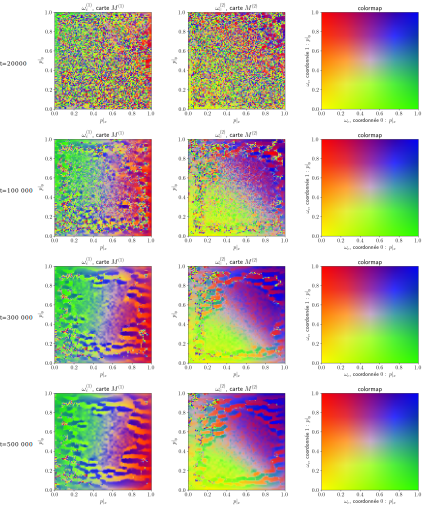
\includegraphics[width=\textwidth]{2SOM_sphere_rc002_evol.pdf}
% 	\caption{\'Evolution des poids contextuels d'une architecture de deux cartes pour $r_c =0.02$. Les poids contextuels évoluent vers une position stable, formant des motifs alternant valeurs hautes et basses des poids contextuels. La zone centrale est constituée de motifs plus resserrés. \label{fig:rc_002}}
% \end{figure}

% \begin{figure}
% 	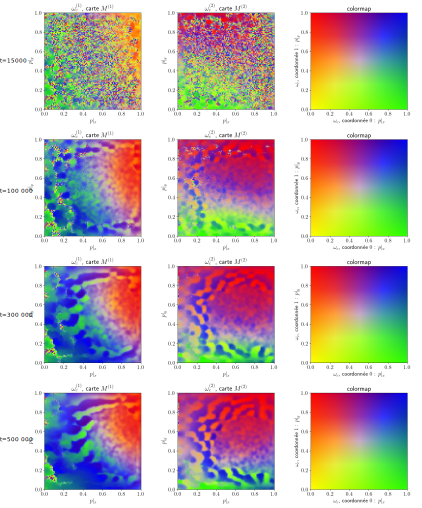
\includegraphics[width=\textwidth]{2SOM_sphere_rc003_evol.pdf}
% 	\caption{\'Evolution des poids contextuels d'une architecture de deux cartes pour $r_c =0.03$. Les poids apparaîssent comme ayant atteint une position stable à l'issue des 500000 itérations.
% 	Les motifs observés sont similaires à ceux observés pour $r_c = 0.02$. \label{fig:rc_003}}
% \end{figure}

\begin{figure}
	\includegraphics[width=\textwidth]{weights_contexte-0-048_rc003.png}
	\caption{\'Evolution des poids contextuels d'une architecture de deux cartes pour $r_c =0.03$. Les poids apparaissent comme ayant atteint une position stable à l'issue des 500000 itérations.
	Les motifs observés sont similaires à ceux observés pour $r_c = 0.02$. \label{fig:rc_003}}
\end{figure}

\begin{figure}[t]
	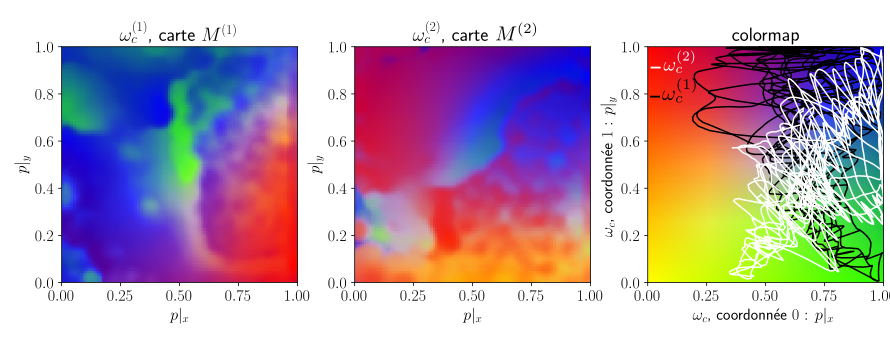
\includegraphics[width=\textwidth]{wc_rc005_grid.pdf}
	\caption{\'Evolution des poids contextuels d'une architecture de deux cartes pour $r_c =0.05$. 
	Nous remarquons que les poids contextuels se déplient sans occuper tout l'espace des positions, ce qui est marqué par la disposition de la grille. Ce dépliement est mis en valeur sous forme de disposition en grille dans l'espace des positions sur la figure de droite : $\w_c\m{1}$ en noir et $\w_c\m{2}$ en blanc. Par ailleurs, nous n'observons pas de convergence claire des poids contextuels~: les grilles noires et blanches continuent d'évoluer après 700 000 itérations.
	Ce comportement rappelle ce qui est observé en 1D. Pour un rayon de voisinage $r_c$ trop grand, les poids contextuels ne forment pas de zones. C'est ce qui est observé dans ce cas en 2D.
	\label{fig:rc_005}}
\end{figure}


% \begin{figure}
% 	\includegraphics[width=\textwidth]{evol_convergence_poids.pdf}
% 	\caption{\'Evolution de la différence moyenne entre les poids externes et contextuels au cours de l'apprentissage d'une architecture de 2 cartes sur une sphère 3D en 4 dimensions. Le calcul de différences est réalisé toutes les 10 000 itérations. Nous avons tracé les courbes pour 4 expériences avec $r_e = 0.2$ et $r_c = 0.02$ ainsi que pour les expériences avec $r_e = 0.2$ et $r_c = 0.05$,$r_e = 0.2$ et $r_c = 0.03$. Nous remarquons que cette différence évolue vers une valeur faible, qu'on attend nulle pour une carte stabilisée. Ici les poids tendent vers une valeur faible qui semble stable. Notons que cela ne montre pas forcément la convergence~: les poids peuvent se déplacer faiblement dans une même direction. Le tracé nous assure simplement que l'évolution des poids est lente en fin d'apprentissage. \label{fig:conv_poids}}
% \end{figure}

\subsection{Convergence de la relaxation \label{par:conv2D}}

Nous nous intéressons ensuite à la convergence de la relaxation sur l'expérience en deux dimensions. 
Nous traçons en figure \ref{fig:relax2D} l'évolution du taux de convergence des tests au cours de l'apprentissage pour des structures de deux cartes en deux dimensions, par le processus décrit au chapitre \ref{chap:relaxation}. Lors de plusieurs phases de test lancées à des itérations $t$ au cours de l'apprentissage, nous comptons le nombre de pas nécessaires à la convergence de la recherche de BMU par relaxation et traçons sur la figure la moyenne de ce nombre de pas de relaxation, à différents temps d'apprentissage $t$.
Nous traçons également le taux d'échantillons d'une phase de test menant à une convergence de la relaxation. On considère que la relaxation n'a pas convergé si le nombre de pas atteint le seuil maximal de 1000 pas fixé par notre étude. Le nombre de pas de relaxation moyen étant observé de 20 pas, 1000 est un seuil que nous jugeons pertinent pour considérer que la relaxation n'a pas convergé.
Nous traçons ces évolutions pour les différentes configurations de paramètres de cartes~: nous avons réalisé trois expériences de mêmes paramètres $r_e=0.2$ et $r_c = 0.02$, une expérience avec $r_c = 0.03$ (cf. figure~\ref{fig:rc_003}, et une avec $r_c = 0.05$ (voir figure \ref{fig:rc_005}).
Dans cette dernière expérience, les poids n'ont pas formé de zones distinctes.
Nous observons sur ce tracé que la relaxation converge bien dans entre 95 et 98 \% des cas tout au long de l'apprentissage, ce qui indique que le BMU trouvé par relaxation a bien un sens de maximum d'activation dans l'architecture (voir chapitre~\ref{chap:relaxation}).
Les valeurs trouvées pour $r_c = 0.05$ sont similaires au cas $r_c = 0.02$, dans lequel les poids ont bien convergé. La relaxation dans des cartes en deux dimensions n'est donc pas liée à la formation de motifs stables dans les poids~: la relaxation trouve un point de convergence dans un cas général de cartes en 2D.
Cette observation est prometteuse pour la construction d'architectures de cartes 2D.

\begin{figure}
	\centering
	\includegraphics[width=0.8\textwidth]{conv_relax_2maps.pdf}
	\vspace{-0.5cm}
	\caption{\'Evolution de la convergence de la relaxation au cours de l'apprentissage. Nous avons réalisé les tracés sur trois expériences générées pour $r_c = 0.02$, sur des entrées aléatoires tirées sur la même distribution, une sphère plongée en 4D. Pour comparaison, nous traçons également l'évolution pour la configuration dans laquelle $r_c = 0.05$, dans laquelle les poids contextuels n'ont pas formé de zones. La relaxation converge en fin d'apprentissage~: la valeur trouvée à l'issue de la relaxation a donc un sens de \og Best Matching Unit \fg{}, également dans les cartes en deux dimensions. \label{fig:relax2D}}
\end{figure}

\section{Organisation des cartes sur des entrées indépendantes \label{par:cub2D}}

Nous nous intéressons enfin à l'organisation d'une architecture de deux cartes prenant des entrées $\inpx\m{1}, \inpx\m{2} \in [0,1]^2 \times 0,1]^2$ indépendantes.
En 1D, nous avions observé deux échelles d'indices dans le choix des BMUs, découpant chaque carte en zones selon la valeur de l'entrée externe. Dans chaque intervalle de ce découpage, les poids contextuels permettent de différencier le BMU selon la valeur de l'autre entrée, formant une sous-carte de toutes les valeurs de $[0,1]$ sur chaque zone de la carte. Nous cherchons à observer si ces zones de BMUs sont encore présentes et si chaque zone permet de cartographier tout l'intervalle $[0,1]^2$.
Les rayons de voisinage sont pris à $r_e = 0.2, r_c = 0.02$, car nous avons constaté dans les expériences précédentes que ces paramètres autorisent la formation de zones.

Les valeurs des poids externes et contextuels sont tracés en figure \ref{fig:2som_cub_wc}.
Les poids externes sont bien dépliés sur l'ensemble des entrées, ce qui est similaire au cas en une dimension.
Les poids contextuels restent par contre centrés autour de $0.5$, mis en évidence par les tracés en blanc et noir sur la carte de coloration à droite de la figure.
Pourtant, nous avons observé que toutes les positions d'une carte sont bien BMU lors des phases de tests. 
Les poids contextuels auraient dû, pour bien cartographier les positions sur l'autre carte, s'étendre sur tout $[0,1]^2$ dans chaque zone.


Ce comportement de moyennage est à rapprocher du comportement limite observé sur une architecture de 10 cartes en une dimension~: nous avons vu que des architectures de 10 cartes apprenant sur 10 entrées 1D indépendantes voient également leurs poids contextuels se moyenner autour de $0.5$ dans chaque carte.
En effet, lorsque les entrées présentent une  dépendance, un nombre fini ou un intervalle réduit de valeurs de $\inpx\m{2}$ seront présentées à l'architecture pour une même valeur de $\inpx\m{1}$. Cela correspond à un nombre réduit de valeurs de $\bmu\m{2}$ donc un nombre réduit d'entrées contextuelles différentes pour $M\m{1}$. 
Les poids contextuels situés autour de la position codant pour $\inpx\m{1}$ s'organisent alors comme une carte des valeurs des entrées contextuelles présentées lorsque $\inpx\m{1}$ est proche de la valeur en question. En une dimension, cette sous carte avait possibilité de s'étendre sur tout l'intervalle de valeurs de $\inpx\m{2}$ possible, formant donc des zones distinctes.
Les connexions entre les n\oe{}uds semblent ici trop rigides pour permettre aux poids contextuels de se déplier dans chaque zone sur tout le carré. Ils prennent donc une valeur centrale.


Ce comportement peut apparaître comme une limite de CxSOM, marquant le fait que les poids contextuels manquent de liberté pour s'organiser. Au contraire, nous pouvons aussi envisager ce comportement comme une capacité de détection de dépendance entre entrées, encore plus marquée sur les cartes 2D que sur les cartes 1D. 

\begin{figure}
	\centering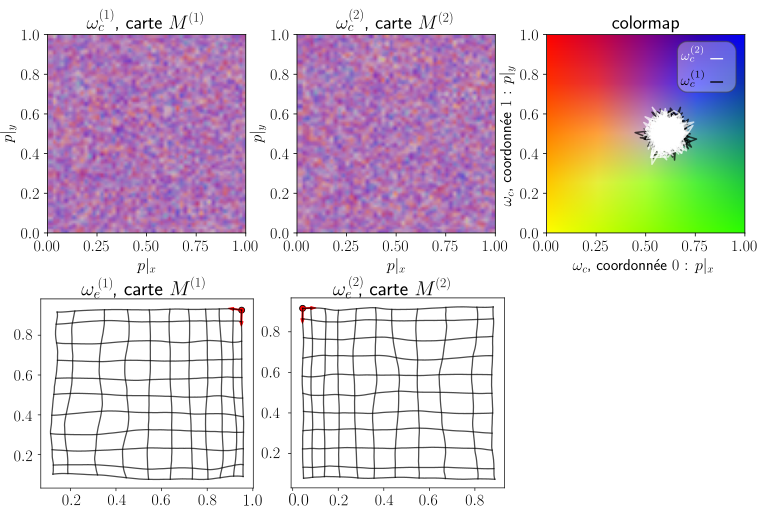
\includegraphics[width=\textwidth]{w_cub_rc002.pdf}
	\caption{En bas~: poids externes des cartes $M\m{1}$ et $M\m{2}$ représentés sous forme de distorsion de la carte après 200000 itérations.
	En haut~: poids contextuels des cartes pour la même itération, représentés sous forme de carte de couleur en deux dimensions. Un pixel situé à la position $p_i,p_j$ prend comme couleur correspondante la valeur 2D de son poids contextuel, associé à une couleur par la carte de coloration représentée à droite de la figure.
	On remarque donc que les poids contextuels ne se déplient pas sur toutes les valeurs prises par les BMU et restent centrés vers le milieu de la carte. \label{fig:2som_cub_wc}}
\end{figure}

\section{Prédiction d'entrée \label{par:pred2D}}

Nous avons vu que les cartes en deux dimensions s'organisent, comme en 1D, de manière à former des zones dans les poids contextuels.  Nous avons également observé que la relaxation converge dans les cartes 2D, donc la dynamique des cartes permet de trouver un BMU correspondant bien à un maximum d'activation.
Nous nous attendons donc à ce qu'une architecture de cartes 2D soit en mesure de générer une prédiction.

Nous vérifions cette capacité de prédiction sur une architecture de trois cartes en deux dimensions. 
Chaque carte prend en entrée externe une paire de coordonnées d'un espace multimodal en 6D. Ces entrées sont situées sur une sphère de dimension 3 plongée dans l'espace en 6D par le même processus de rotation qu'en 4D. $U$ est donc toujours une variable $2D$. 
Dans cette configuration, la connaissance de deux entrées sur trois et du modèle détermine la troisième~: la prédiction est donc envisageable.
Nous prenons $r_e = 0.2$ et $r_c = 0.02$ et des cartes de taille $100 \times 100$. Les cartes ont été entraînées sur 250 000 itérations, à l'issue desquelles les poids externes contextuels ont atteint une position stable.

Nous traçons d'abord les poids externes et contextuels des trois cartes en figure~\ref{fig:3som_w}.
L'organisation des poids contextuels conduit à la présence de motifs très semblables à ceux observés sur une architecture de deux cartes.
Nous réalisons une étape de prédiction à la fin de l'apprentissage lors de laquelle une carte ne reçoit plus d'entrée externe, par exemple ici $M\m{2}$.
La valeur de $\w\ext\m{2}(\bmu\m{2})$ est alors utilisée comme prédiction de l'entrée $\inpx\m{2}$.
La figure~\ref{fig:3som_pred} indique la valeur prédite en fonction de l'entrée $\inpx\m{2}$. 
Les valeurs de $\inpx$ et $\w_e$ étant 2D, nous avons représenté séparément chaque dimension. Cette expérience montre que la prédiction est correctement réalisée, donc que l'architecture a appris le modèle des entrées 2D. Nous observons les mêmes capacités de prédiction pour $M\m{1}$ et $M\m{3}$.
L'erreur de prédiction observée dans cet exemple est cependant très élevée par rapport à l'échelle de quantification vectorielle possible~: chaque carte possède 10000 n\oe{}uds, on aurait pu s'attendre à une meilleure précision.
L'organisation induite par le modèle CxSOM rend de nombreux n\oe{}uds inutilisés en 1D comme en 2D, les n\oe{}uds morts. Ces n\oe{}uds sont utiles pour l'organisation en tant que zones de transition, mais n'encodent pas de valeur pour la quantification vectorielle de l'entrée externe et pour la prédiction. Ces n\oe{}uds morts sont encore plus nombreux dans les cartes 2D que les cartes 1D car ils s'étendent sur les deux dimensions. On a donc globalement une fuite massive d'unités d'encodage dans le modèle CxSOM. Cela pourrait expliquer le fait que la prédiction est mal réalisée en 2D~: peu de n\oe{}uds encodent véritablement les valeurs d'entrées.
Ce comportement sera donc à évaluer sur d'autres distributions d'entrée afin de vérifier la capacité de prédiction d'une architecture de cartes 2D.

\begin{figure}
		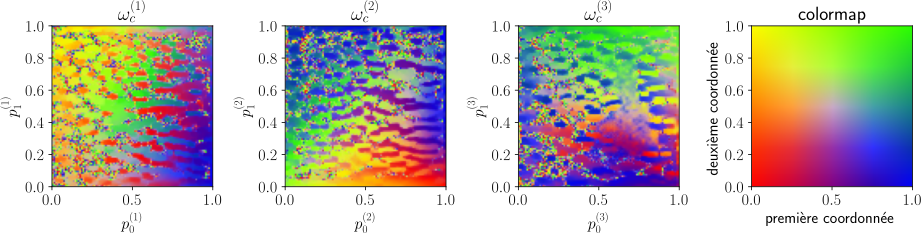
\includegraphics[width=\textwidth]{3SOM_S_wc_239999.png}
		\caption{Tracés des poids externes dans l'espace des entrées (en bas) et des deux couches de poids contextuels de chaque carte sous forme de carte de coloration. L'angle $(0,0)$ d'une carte est marqué par le point rouge. Les motifs formés par les poids contextuels sont similaires à ceux observés sur deux cartes. \label{fig:3som_w}}
\end{figure}

\begin{figure}
\centering\includegraphics[width=0.8\textwidth]{3SOM_error_closed.pdf}
\caption{Tracé de l'erreur de prédiction $\w_e\m{2}(\bmu\m{2})$ en fonction de la valeur théorique de $X^{(2)}$, non présentée à l'architecture, dans une architecture de trois cartes 2D prenant des entrées $X^{(i)}$ en deux dimensions $[X^{(i)}|_x, X^{(i)}|_y]$. Nous traçons sur une ligne, pour chaque entrée, les dépendances entre chacune des dimensions
lorsque la carte $M^{(2)}$ ne reçoit pas d'entrée externe. Les cartes $M^{(1)}$ et $M^{(3)}$ ayant une activité externe, le graphique montre que la quantification vectorielle est bien réalisée dans ces cartes. La carte $M^{(2)}$ est uniquement activée par les connexions contextuelles venant de $M^{(1)}$ et $M^{(3)}$. La figure centrale montre que la prédiction est correctement réalisée, mais que l'erreur de prédiction est élevée. \label{fig:3som_pred}}
\end{figure}


\section{Conclusion}

Les expériences proposées dans ce chapitre sur les cartes en deux dimensions donnent une idée des comportements auxquels on peut s'attendre dans un cas plus général d'architecture.
Ces expériences nous ont également permis d'utiliser la méthode d'étude de carte proposée tout au long de cette thèse et constituent une première utilisation des indicateurs proposés au chapitre précédent.


Nous avons d'abord observé que l'émergence de zones de poids contextuels est une propriété qui se transpose bien sur des cartes en deux dimensions. Ces zones constituent donc un comportement systématique des architectures CxSOM.
La formation de ces zones permet, comme sur des cartes 1D, de séparer les valeurs de $U$ en fonction des positions des BMUs. $U$ est une fonction du BMU dans chacune des cartes.
Cette séparation est correctement évaluée par le ratio de corrélation.
Nous avons observé que comme sur les cartes 1D, les zones dépendent du rapport entre les rayons de voisinage externes et contextuels et ne se forment qu'à partir d'une certaine valeur pour ce rapport.
Comme en 1D, la relaxation converge en fin d'apprentissage et le BMU 2D a donc un sens dans une carte, ce que nous avions également observé au chapitre \ref{chap:relax} pour des cartes 1D et 2D apprenant sur des entrées 1D.
Enfin, nous avons observé une bonne capacité de prédiction d'une modalité manquante sur une disposition d'entrée en sphère dans un espace 6D.

Une architecture de cartes en deux dimensions présente donc des propriétés similaires à celles observées sur les cartes 1D et généralise le comportement observé en 1D.
Cette généralisation est soumise à quelques contraintes supplémentaires aux cartes 1D.
La convergence des poids, contrairement aux cartes en une dimension, n'est pas assurée pour tous paramètres d'apprentissage et constitue un point à vérifier lors de la construction d'architectures de cartes en deux dimensions.
Par ailleurs, nous avons déplié les poids externes lors d'une étape d'initialisation afin de s'assurer que la carte 2D ne présente pas de point de torsion. La robustesse de l'algorithme CxSOM, en particulier de la relaxation, sur des cartes \og mal dépliées \fg{} peut constituer un point d'étude pour une éventuelle application de l'algorithme.
Enfin, dans le cas ou les entrées sont indépendantes, dans lequel une même position de BMU pour $M\m{1}$ correspond à toutes les positions de BMUs $[0,1]^2$ pour $M\m{2}$, les poids contextuels ne se déplient pas localement de façon à cartographier tout l'espace $[0,1]^2$.
Ce comportement se rapproche du cas limite observé sur les architectures de 10 cartes 1D. 
Les cartes 2D ont ainsi le même comportement que les cartes 1D lorsque les entrées sont indépendantes~: les poids contextuels se moyennent autour d'une position centrale et l'activité liée à ces poids contextuels n'intervient alors plus dans le calcul de l'activité globale.
Ce comportement apparaît comme une capacité de l'architecture à détecter automatiquement les relations entre entrées. Cependant, il peut aussi être un facteur limitant l'apprentissage d'entrées lorsque le modèle $U$ est de grande dimension, marquant une trop grande rigidité des poids contextuels. 

Le passage de 1D à 2D apporte également une diversité dans les comportements d'apprentissage observés en 1D~: la forme des motifs spatiaux formés par les poids contextuels est plus variable que dans le cas des cartes en une dimension.
Cela peut être un atout pour le modèle, car cela laisse la porte ouverte à des comportements plus complexes sur des grandes architectures cartes 2D~; mais cela nécessite plus d'outils pour une compréhension des mécanismes d'apprentissage.
Ainsi, il sera pertinent d'étudier le comportement d'une architecture de cartes d'un point de vue macroscopique pour la suite des travaux, à partir d'indicateurs et de représentations portant sur la réponse globale d'une architecture, et non seulement à l'échelle d'une carte comme nous l'avons fait dans cette thèse.

\ifSubfilesClassLoaded{
    \printbibliography
    %\externaldocument{../main.tex}   
}{}
\end{document}



% PLAN


% Convergence des poids :
% - Dépend des paramètres, contrairement à la carte en 1D on n'arrive pas forcément dans une position stable
% - Rc = 0.02 : point fixe, avec une partie 
% - Chaque expérience différente : grande dépendance aux conditions initiales. 